\chapter{Background \label{cha:chapter2}}

In order to set context of underlying thesis work, this chapter provides background information on virtualization technologies and embedded systems with special emphasis on the ARM platforms. A brief overview of PHIDIAS, the static hypervisor in question is also given at the end of this chapter.

\section{Introduction to Virtualization \label{sec:tech}}
Virtualization is a mechanism of providing abstraction between computer hardware systems and softwares running on them, allowing us to create multiple computing environments and exploiting the resource isolation on a single physical platform. It basically gives a logical view of multiple operating environments running on a single hardware. With the recent developments in virtualization, there has been huge investments in organizations over this technology to improve the efficiency and availability of resources and applications. Enterprises are giving up the old \textbf{one server, one application} model and gaining benefits from server consolidation provided by virtualization. This technology has dramatically changed the IT landscape by reducing underlying expenses and providing economies of scale and greater efficiency.

\subsection{History of Virtualization\label{sec:history}}
History of virtualization dates back to 1950's when the Compatible Time Sharing System (CTSS) was developed at MIT on IBM 704 series computer. The supervisor program of CTSS handled console I/O, scheduling of foreground and background (offline-initiated) jobs, temporary storage and recovery of programs during scheduled swapping, monitor of disk I/O, etc. The supervisor had direct control of all trap interrupts \cite{introtousevirtualization}.\\
\\
In the fall of 1963, MIT's Project MAC was founded with the main purpose of designing and implementation of a better time sharing system than CTSS. After IBM lost the bid to General Electric's GE 645, it created a number of virtual machine systems e.g, the CP-40 (developed for a modified version of IBM 360/40), the CP-67 (developed for the IBM 360/67), VM/370, and many more. We can roughly say that Virtual Machine technology was brought to users with the introduction of the CP-67 hypervisor on the S/360 Model 67 processor. In 1999, VMware introduced virtualization on x86 platforms. Since then, many vendors like Microsoft, Citrix etc had followed VMware and technology has been evolved with the advances in hardware architectures. 
\\
\\
\subsection{Benefits of Virtualization\label{sec:uses}} 
For many years, server virtualization was considered one of the biggest advantages of using virtualization technology and VMware enjoyed a long run as a king of x86 server virtualization. However, many players e.g. Citrix and Microsoft started to gain ground in this field by offering additional middle-ware and desktop virtualization solutions. Over the past several years, there has been huge improvements in this domain and vendors are continuously innovating to increase capabilities of virtualized systems and developing their management tools.\\
\\
Following are some of the main benefits of using virtualization technology \cite{reasonstousevirtualization}:

\subsubsection{Better utilization of resources \label{sec:resource optimization}}
With virtual machines, resources of computing platforms can be used in an optimal manner to achieve better performance. Servers used in data centers typically have large resource capabilities. However, they are not fully utilized because of small number of connected users or less demanding applications. Virtualization of hardware allows on-demand resource allocation leading to efficient use of computing power, storage space and network bandwidth. In addition to on-demand usage of resources, virtualization also provides resource isolation between virtual machines. Each virtual machine can run software without affecting execution of other guests. 

\subsubsection{Consolidation \label{sec:Consolidation}}
For many years, individual servers have been dedicated to run single applications. For less demanding applications, computing capabilities would be wasted. With the advent of virtualization, organizations are now deploying several applications on single servers using only a small amount of processing power. Server consolidation has led to dramatic reduction in need of floor space, HVAC, A/C power, and co-location resources which has caused cost reduction and efficient power consumption.

\subsubsection{Security and Isolation\label{sec:security}}
Virtualization allows running multiple virtual machines in an isolated secure environment. All privileged calls made by guests are analyzed by hypervisor to provide safety against vulnerabilities and attacks. Exceptions and traps of one virtual machine are handled by hypervisor layer, isolating other virtual machines from the resulting affects. Virtualization regulates access permissions to the programs with reduced privileges from misusing resources. 

\subsubsection{Migration and Increased Uptime\label{sec:migration}}
Migration is the process of moving a running virtual machine from one place to another without affecting overall system. With virtualization, organizations can get better performance and reliable systems. It also increases uptime of servers and applications. Virtual machines can easily be backed up and restored for speedily recovery from computing disasters.

\subsection{Overview of Hypervisors\label{sec:aaa}}

A virtualization layer that separates the service request from underlying physical delivery of that request is called virtual machine monitor (VMM) or hypervisor. Hypervisor allows multiple operating systems to run concurrently within virtual machines on a single computer and provides dynamic allocation and sharing of physical resources e.g. CPU, memory, storage and I/O devices \cite{hypervisor1}. It is an abstraction layer that enables communication between hardware and virtual machines \cite{hypervisor2}. Figure \ref{Virtualization1} provides an illustration of virtualization architecture.

\begin{figure}[htb]
\centering
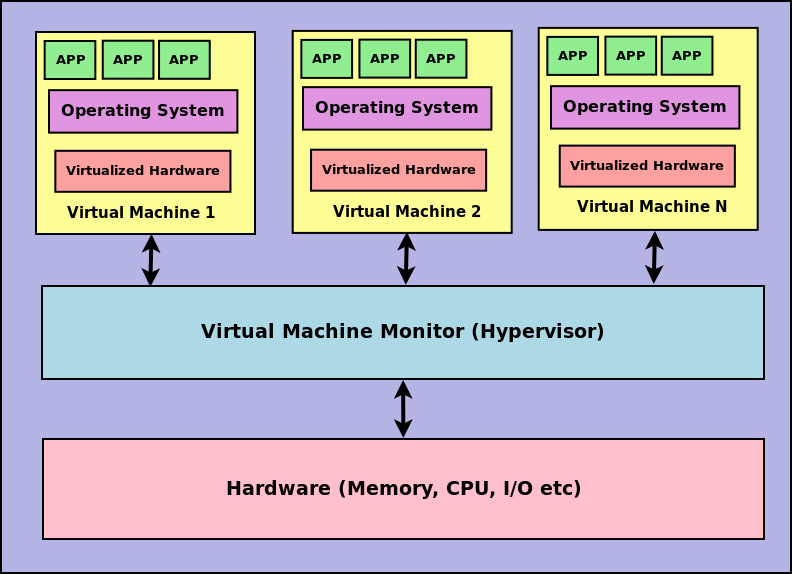
\includegraphics[width=10cm]{Virtualization_Abstraction}
\caption{Virtualization Framework}
\label{Virtualization1}
\end{figure}

In 1974, Popek and Goldberg published an article `Formal Requirements for Virtualizable Third Generation Architectures' in which they described the following requirements of a hypervisor for efficient virtualization \cite{popek_goldberg_1973}:
\begin{itemize}
	\item Virtualization environment provided by hypervisor should be native system so that program behaves in a similar fashion.
	\item Virtualized resources should be shared with security controls to protect from any threats and performance interference.
	\item Good support to handle privileged instructions should be provided in order to avoid performance degradation.
\end{itemize}
Keeping in view the above requirements, different types of hypervisors have been introduced in market which are categorized into two main classes as shown in Figure \ref{VirtualTypes}
\begin{figure}[htb]
	\centering
	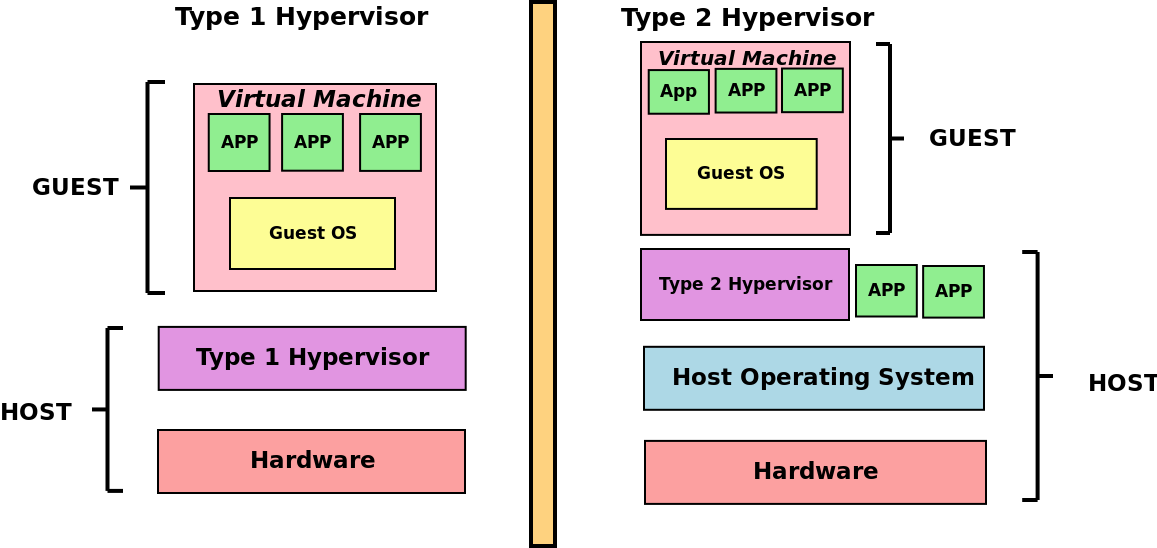
\includegraphics[width=10cm]{Hyper1vsHyper2}
	\caption{Type-1 vs Type-2 Hypervisor}
	\label{VirtualTypes}
\end{figure}
\subsection{Types of Hypervisors\label{sec:bbb}}
Following are two types of hypervisors:
\begin{itemize}
	\item \textbf{Type-1 or bare-metal} hypervisor sits directly on hardware and manages virtual machines on top of it. It is also called bare-metal hypervisor. Examples of type 1 hypervisors are \textit{VMware vSphere/ESXi, Microsoft Windows Server 2012 Hyper-V, Citrix XenServer, Red Hat Enterprise Virtualization (RHEV) and KVM} \cite{hypervisor2}.
	\item \textbf{Type-2 or hosted} hypervisor runs on host operating system to manage virtual machines where hosted operating system provides hardware configuration. VirtualBox and VMware	Workstation are examples of type-2 hypervisors.
\end{itemize}
According to IBM, type-1 hypervisors provide higher performance, availability, and security than type-2 hypervisors. IBM recommends that type-2 hypervisors should be used ,mainly on client systems, where efficiency is less critical or on machines where support for a broad range of I/O devices is important and can be provided by the host operating system \cite{searchservervirtualization}.
\\
Since bare-metal hypervisor has direct access to the hardware resources rather than going through
an operating system, it is considered to be more efficient than a hosted architecture and delivers greater scalability, robustness and performance \cite{hypervisor1}. 

\subsection{State of the Art Hypervisors\label{sec:comp}}
Over the past decade, virtualization technology has gone from small deployments to full blown IT infrastructure development. Technology makers have shifted their focus from operating systems, having one-to-one relationships with hardware, towards developing virtualized machines running on a single platform. Talking about big players in this industry, VMware is a dominating contender. Other key players include Citrix XenServer, Microsoft Hyper-V, RHEV, Oracle's Solaris Zones, LDoms and xVM, Amazon's Elastic Compute Cloud (EC2), Google Ganeti cluster virtual server management software tool and Virtual Bridges' VERDE product \cite{players}. In 2011, Younge, Andrew J., et al. \cite{younge2011analysis} provided a comparison of main virtualization solutions as illustrated in Figure \ref{comparison}.
\begin{figure}[!htbp]
	\centering
	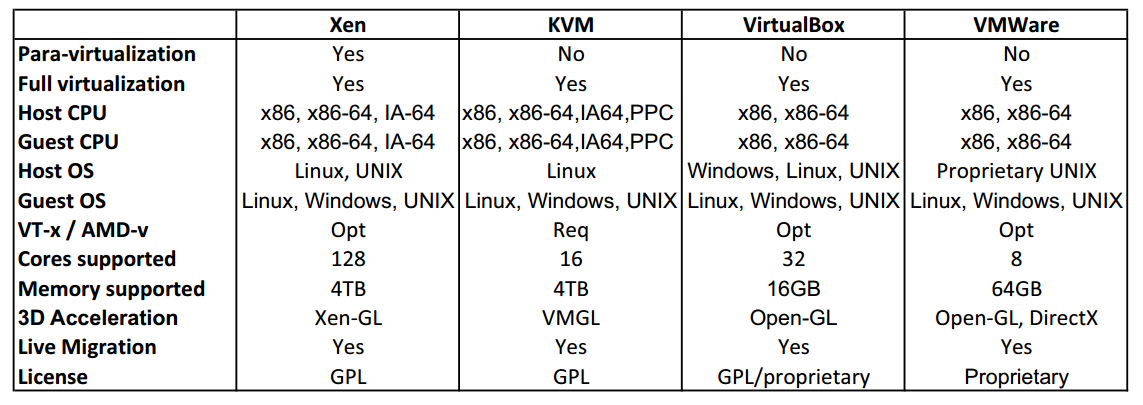
\includegraphics[width=10cm]{Comparison}
	\caption{A comparison chart between Xen, KVM, VirtualBox, and VMWare ESX. Taken from from "Analysis of virtualization technologies for high performance computing environments" by Younge, Andrew J., et al, 2011, p11}
	\label{comparison}
\end{figure}

\section{Embedded Systems \label{sec:standard}}
Embedded systems are composed of simple devices used to perform small and dedicated functions with specific hardware and software constraints i.e. low memory and efficient power usage, long battery life, smaller footprint, lower weight with reduced cost and reliability \cite{koopman1990design}. According to Steve Heath, author of book `Embedded System Designs' \cite{heath_2005}:

\textbf{\textit{`An embedded system is a microprocessor-based system that is built to control a function or a range of dedicated functions and is not designed to be programmed by the end user in the same way as general purpose PC is'}}. 
\\
\\
He had described distinctive capabilities of embedded systems leading to wide spread use of microprocessors today. Some of the main features are given below:
\begin{itemize}
	\item \textbf{Replacement of discrete logic circuits} to reduce the time and cost of developing new products by changing program code to process data in embedded systems.
	\item \textbf{Upgrading systems} by changing the software while keeping the hardware same thus reducing the cost of production and testing of software.
	\item \textbf{Providing easy maintenance upgrades} for adding new functionalities and resolving bugs by reprogramming the software without modifying the hardware.
	\item \textbf{Protecting intellectual property} by encapsulating the functionality of system by burning firmwares on chips making it harder to reverse engineer it.
\end{itemize}

In short, embedded systems are designed for performing a fixed or a few number of dedicated functions. For running other types of general applications, general purpose computers can be used. General purpose computers are also re-programmable by end users while embedded systems are not. As far as speed and size are concerned, embedded systems are smaller in size and run at fixed optimized speed while general purpose computers are bigger in size with mostly predictable speeds.
\\
\\
However, with the advances in hardware technology and virtualization, embedded devices can now run general purpose operating systems or application with little or no knowledge of hardware constraints. Although safety critical systems are far more restricted that so-called modern embedded systems, virtualization could still bring advantages, by increasing their safety, reliability and security \cite{aguiar_hessel_2010}.

\subsection{Virtualization on Embedded Systems\label{sec:itu}}
Adding a hypervisor to an embedded system adds flexibility and higher-level capabilities, morphing the embedded device into a new class of system \cite{ibm}. Embedded devices are ubiquitous and are major part of our lives today. Their common use is in real time applications with hardware and software constraints. However, a recent trend seen today is to use these devices in virtualized systems. One of the reasons is that users want to run applications developed originally for general purpose OSes and still desire to achieve real time responsiveness. There is where virtualization comes in handy. With virtualization, we can enable concurrent execution of real time OS (RTOS) and application OS(Windows, Linux etc) on same hardware. Another benefit will be security which can be achieved by encapsulating vulnerable application OS in a separate VM, thus preventing access to the rest of system.
\\
\\
In a nutshell, there are many uses of deploying virtualization on embedded systems and with the development in multi-cores technology, we can expect innovative solutions in future embedded systems. 

\subsection{ARM Embedded Platforms\label{sec:itu}}
Since the target processor used in this thesis was ARMv8 Cortex-A53, this section will provide a brief introduction on ARM, in general, and ARMv8 architectures, in particular.

\subsubsection{Introduction to ARM Architecture\label{sec:arch}}
ARM, originally \textbf{Acorn RISC Machine}, later \textbf{Advanced RISC Machine}, is a family of reduced instruction set computing (RISC) architectures for computer processors, configured for various environments \cite{wikipedia_2017}. ARM has the following RISC architectural features \cite{ARM}:
\begin{itemize}
	\item A uniform register file load/store architecture, where data processing operates only on register contents, not directly on memory contents. 
	\item Simple addressing modes, where all load/store addresses are only determined from register contents and instruction fields.
\end{itemize}
With the increase in demands of new functionality and emerging market trends, ARM architecture has evolved over time. ARM processors are basically used to achieve high-performance at lower cost with efficient power consumption. There is a concept of \textbf{profiles} in ARM architecture describing different versions to be used in multiple market segments \cite{ARM}. Table \ref{tableARM} highlights different profiles of ARM architecture.
\begin{table}[!htbp]
\centering
\begin{tabular}[t]{|L{4cm} |L{8cm}|}
\hline
Profile & Description \\
\hline
Architecture (`A') profile  & Provides high performance and 
usually used in mobile and enterprise markets  \\
\hline
Real-Time (`R') profile & Provides real time performance and
 used in embedded applications for automotive and industrial control. \\
\hline
Microcontroller (`M') profile & Provides time critical and  real time performance for microcontroller market\\
\hline
\end{tabular}
\caption{Description of ARM profiles}
\label{tableARM}
\end{table}

\subsubsection{ARM processor modes and Registers\label{sec:processor_modes}}
There are two categories of ARM processor modes i.e. privileged and non-privileged modes. Privileged mode is used to handle exceptions or to access system resources while non-privileged mode has restricted permissions to use protected resources. Each processor mode uses its own stack and a subset of registers. Table \ref{tab:modes} shows different processor modes supported by ARM architecture.
\begin{table}[!htbp]
	\centering
	\begin{tabular}[t]{|L{3cm} |L{8cm}|C{2cm}|}
		\hline
		\multicolumn{1}{|c|}{\textbf{Modes}}  &	\multicolumn{1}{|c|}{\textbf{Description}}    & 	\multicolumn{1}{|c|}{\textbf{Category }  }    \\ 
		\hline

		User                 & Normal program execution  & Privileged  \\\hline

		Fast interrupt (FIQ) & Handles fast interrupts  &     \\
        \cline{1-2}
		Interrupt (IRQ)      & Handles regular interrupts  &      \\
\cline{1-2}
		Supervisor           & Handles operating system functions. System enters into this mode when the power is applied.     &    \multirow{5}{*}{\centering Privileged}   \\
\cline{1-2}
		Abort                & Handles Data Aborts and Prefetch Aborts and helps to implement virtual memory        &      \\
\cline{1-2}
		System               & Handle operating systems function  in user mode and uses same registers as User mode    &      \\
\cline{1-2}
		Undefined            & Handles Undefined instructions with the support of software emulation of hardware co-processors &     \\
		\cline{1-2}
		Monitor & Provides support of switching between secure and  non-secure states available on processors with security extensions & \\
			\hline
	\end{tabular}
	\caption{Description of ARM processor modes}
	\label{tab:modes}
\end{table}
In all ARM processors, the following registers are available and accessible in
any processor mode \cite{arm_information_center}:
\begin{itemize}
	\item 13 general-purpose registers R0-R12
	\item 1 Stack Pointer (SP)
	\item 1 Link Register (LR)
	\item 1 Program Counter (PC)
	\item 1 Application Program Status Register (APSR)
\end{itemize}
ARM processor has total of 37 registers (40 with security extension implementations) arranged in partially overlapping banks which help to context switch rapidly. Figure \ref{ARM_Registers} shows the organization of general purpose registers of different ARM processor modes.

\begin{figure}[!htbp]
	\centering
	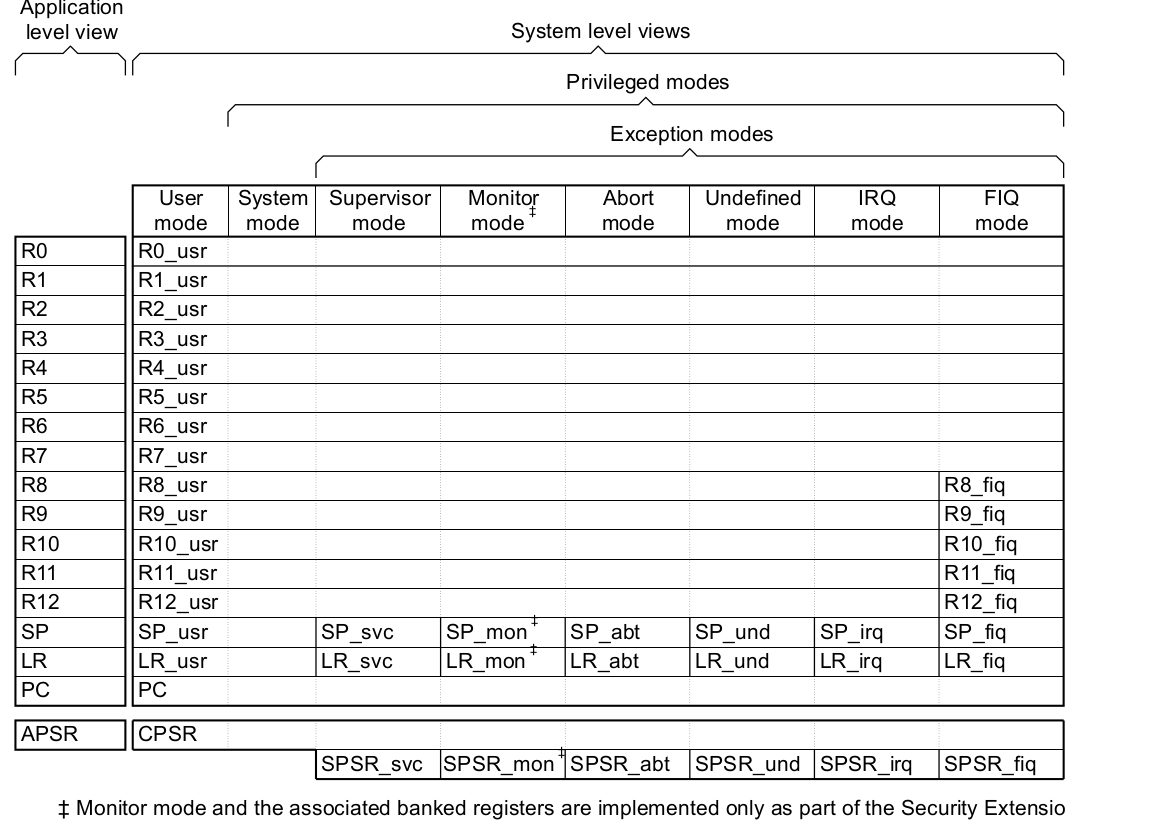
\includegraphics[width=10cm]{ARM_Registers}
	\caption{Organization of ARM registers for different processor modes. Taken from \cite{arm_information_center}}
	\label{Virtualization}
\end{figure}

\subsection{ARMv8-A Architecture\label{sec:armv8}}
The basic feature of ARMv8 architecture is that it supports both 32-bit (AArch32) and 64-bit (AArch64) execution states \cite{armv8}. In AArch64 state, the instructions can access both the 64-bit and 32-bit registers. However, in AArch32 state, the instructions can only access the 32-bit registers, and not the 64-bit registers \cite{states}. For this thesis, AArch64 execution state has been used which supports up to four Exception levels, EL0 - EL3 and has 64-bit virtual addressing. Table \ref{exeception_model} shows the description of exception model levels.
\begin{table}[!htbp]
	\centering
	\begin{tabular}[t]{|L{4cm} |L{8cm}|}
		\hline
		Exception Level & Description \\
		\hline
		 EL0 &  Applications\\
		\hline
		EL1 & OS kernel and associated privileged functions \\
		 \hline
		 EL2& Hypervisor  \\
		 \hline
		 EL3 &  Secure Monitor\\
		 \hline
	\end{tabular}
	\caption{Description of ARMv8 Exception Model Levels}
	\label{exeception_model}
\end{table}
Cortex-A53 processor is a mid-range, low-power processor which implements the ARMv8-A
architecture with  Generic Interrupt Controller (GIC) v4 and ARM Generic Timer  \cite{cortexA53}.


\subsubsection{ARMv8-A Memory Management\label{sec:armv8_mem}}
Memory management unit (MMU) is a hardware that performs virtual address to physical address mapping. It does this by controlling the walk and access of translation tables held in main memory. Transalation tables hold virtual to physical address mappings and memory attributes which are then loaded into the Translation Lookaside Buffer (TLB) when a location is accessed \cite{cortexA53}.
With MMU enabled in system, applications can run independently in their own virtual address space without having the knowledge of physical addresses used by hardware. Figure \ref{mmu} shows the MMU hardware in ARM architecture.
\begin{figure}[!htbp]
	\centering
	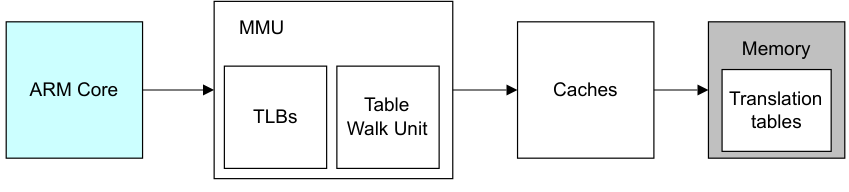
\includegraphics[width=10cm]{mmu}
	\caption{Sructure of ARM MMU. Taken from \cite{mmu}}
	\label{mmu}
\end{figure}

Lets see what type of addressing scheme is used by ARMv8 platform in this thesis. The target hardware is using 48-bit virtual addresses with 4KB page size and four level of address lookup. The 48-bit address has nine bits for each level of translation with the last 12 bits of original address defining the offset within the 4KB page size. Each level of translation lookup table has 512 entries.
Bits 47:39 of virtual address index into the 512 entry L0 table. Each of these table entries spans a 512 GB range and points to an L1 table. Within that 512 entry L1 table, bits 38:30 are used as index to select an entry and each entry points to either a 1GB block or an L2 table. Bits 29:21 index into a 512 entry L2 table and each entry points to a 2MB block or next table level. At the last level, bits 20:12 index into a 512 entry L2 table and each entry points to a 4kB block \cite{translation}. Figure \ref{translation} shows the division of 48 bit address for four levels of translation lookup used by MMU in Cortex-A53 processor.

\begin{figure}[!htbp]
	\centering
	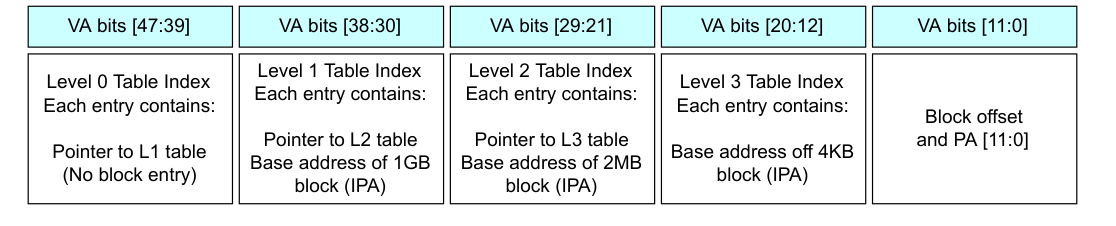
\includegraphics[width=10cm]{translation}
	\caption{48-bit address translation lookup for 4KB granule size on ARMv8 architecture. Taken from \cite{translation}}
	\label{translation}
\end{figure}


\subsection{Device Emulation on ARMv8-A Embedded Systems\label{sec:3gpp}}
ARMv8-A architecture supports virtualization by implementing EL2 execution state for running hypervisor. Hypervisor in EL2 state is responsible for executing multiple guests in non-secure EL1 state. Each guest can run user applications in EL0 state which is also non-secure. Address translation occurs in two stages for virtualized guests. Stage 1 translation converts virtual addresses to intermediate physical address (IPA) which is managed by virtual machine in EL1 state. Stage 2 translation converts IPA to physical address which is managed by hypervisor in EL2 state. These IPA are treated as actual physical addresses by guest OSes. ARM virtualization extensions have made generic timers (GT) and the generic interrupt controller (GIC) virtualization aware. Hence CPU, memory, interrupts and timers can be emulated using full hardware virtualization. However, for I/O devices, para-virtualized drivers could be used.\\
\\
There are two ways of I/O virtualization. First method involves rewriting of device drivers in VMM as shown in Figure \ref{VMMIO}. It provides high performance but it increases the chances of introducing bugs in hypervisor code and has high engineering costs. Other method is to use para-virtualized device drivers in guest OS as shown in Figure \ref{Host_io}. It has lower engineering costs and more fault tolerance but it has performance overheads.



\begin{figure}[!htbp]
\begin{center}
\begin{tikzpicture}
\node at (2,-6) [rectangle, draw=black, thick,line width=2.5pt, rounded corners, fill=white!5, minimum height = 2cm, minimum width = 6cm, anchor=south west, text width=7.8cm, path picture={\node at (1.8, -1.1){ 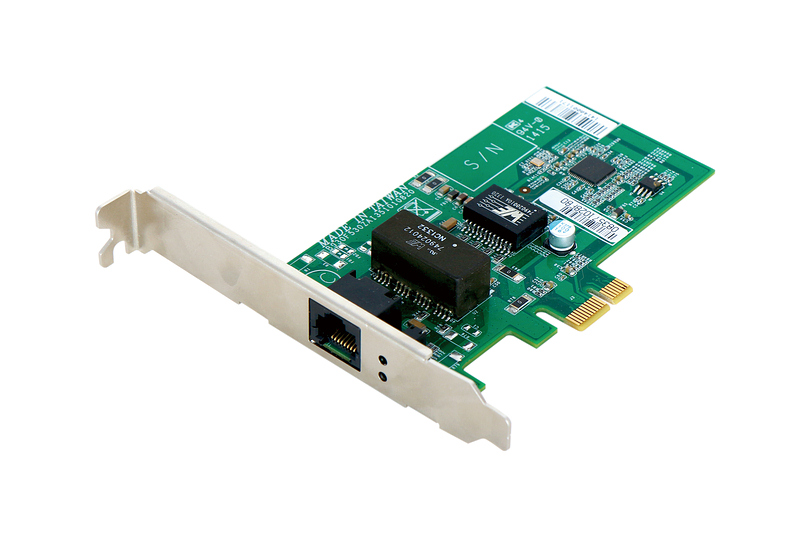
\includegraphics[width=3.5cm]{NIC}};, \node at (4.8, -1.1){ 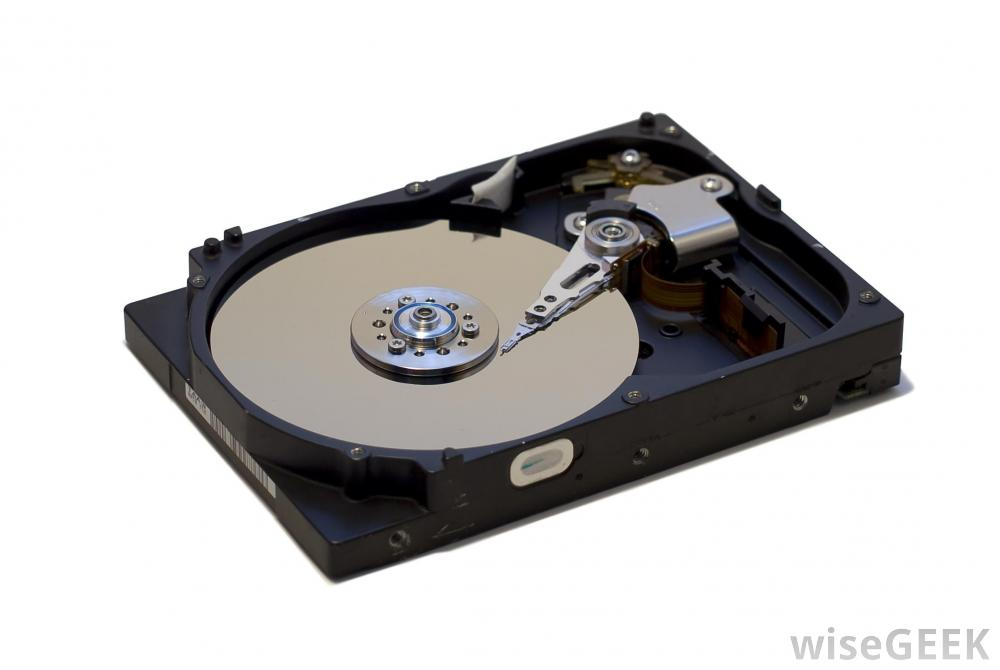
\includegraphics[width=3.5cm]{disk}};} ] (ntw) {Hardware}  ;
\node at (2,-4) [rectangle, draw=black, thick,line width=2.5pt, rounded corners, fill=white!5, minimum height = 2cm, minimum width = 6cm, anchor=south west, text width=7.8cm] (nta) {Hypervisor}  ;
\node at (4.8,-3.7) [rectangle, draw=black, thick,line width=2.5pt, rounded corners, fill=white!5, minimum height = 1.4cm, minimum width = 1.1cm, anchor=south west, text width=1.8cm] (nta1) {Network Device Driver}  ;
\node at (7.8,-3.7) [rectangle, draw=black, thick,line width=2.5pt, rounded corners, fill=white!5, minimum height = 1.4cm, minimum width = 1.1cm, anchor=south west, text width=1.8cm] (nta2) {Block Device Driver}  ;
\node at (4.8,-1.7) [rectangle, draw=black, thick,line width=2.5pt, rounded corners, fill=white!5, minimum height = 1.4cm, minimum width = 1.1cm, anchor=south west, text width=1.8cm] (nta3) {Guest OS}  ;
\node at (7.8,-1.7) [rectangle, draw=black, thick,line width=2.5pt, rounded corners, fill=white!5, minimum height = 1.4cm, minimum width = 1.1cm, anchor=south west, text width=1.8cm] (nta4) {Guest OS}  ;
\end{tikzpicture}
\end{center}
\caption{I/O Virtualization in Hypervisor (VMM)}
\label{VMMIO}
\end{figure}

\begin{figure}[!htbp]
\begin{center}
\begin{tikzpicture}

\node at (2,-6) [rectangle, draw=black, thick,line width=2.5pt, rounded corners, fill=white!5, minimum height = 2cm, minimum width = 6cm, anchor=south west, text width=7.8cm, path picture={\node at (1.8, -1.1){ 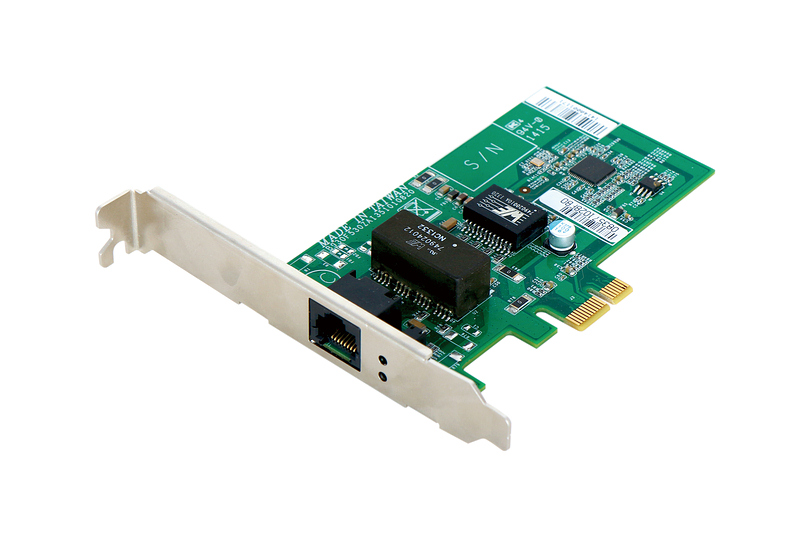
\includegraphics[width=3.5cm]{NIC}};, \node at (4.8, -1.1){ 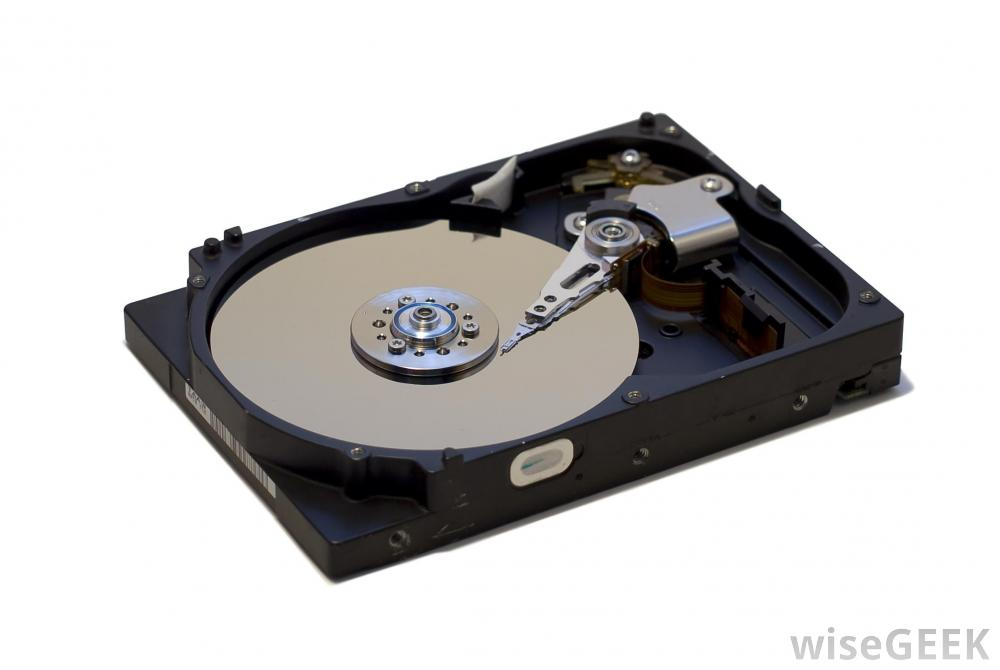
\includegraphics[width=3.5cm]{disk}};} ] (ntw) {Hardware}  ;
\node at (2,-4) [rectangle, draw=black, thick,line width=2.5pt, rounded corners, fill=white!5, minimum height = 2cm, minimum width = 6cm, anchor=south west, text width=7.8cm] (nta) {Hypervisor}  ;
\node at (2,-1.7) [rectangle, draw=black, thick,line width=2.5pt, rounded corners, fill=white!5, minimum height = 3.4cm, minimum width = 3cm, anchor=south west, text width=4cm] (nta3) {\begin{minipage}[t][3.1cm]{4.5cm}{Privelged Guest or Host OS} \end{minipage}}  ;
\node at (2.5,-0.9) [rectangle, draw=black, thick,line width=2.5pt, rounded corners, fill=white!5, minimum height = 1.4cm, minimum width = 1cm, anchor=south west, text width=1.3cm] (nta1) {Network Device Driver}  ;
\node at (4.35,-0.9) [rectangle, draw=black, thick,line width=2.5pt, rounded corners, fill=white!5, minimum height = 1.4cm, minimum width = 1.3cm, anchor=south west, text width=1.3cm] (nta2) {Block Device Driver}  ;
\node at (6.5,-1.7) [rectangle, draw=black, thick,line width=2.5pt, rounded corners, fill=white!5, minimum height = 1.4cm, minimum width = 1.1cm, anchor=south west, text width=1.1cm] (nta3) {Guest OS}  ;
\node at (8.2,-1.7) [rectangle, draw=black, thick,line width=2.5pt, rounded corners, fill=white!5, minimum height = 1.4cm, minimum width = 1.1cm, anchor=south west, text width=1.1cm] (nta4) {Guest OS}  ;
\end{tikzpicture}
\end{center}
\caption{I/O Virtualization in privileged Guest VM or Host OS }
\label{Host_io}
\end{figure}

With ARM virtualization extensions, virtualization of I/O devices has become more efficient. The main features of these extensions include introduction of a new higher privileged \textbf{Hypervisor} execution mode than \textbf{Supervisor} mode, mechanisms to aid interrupt handling, the provision of a System MMU (SMMU) to aid memory management, two levels of address translation and support of hardware acceleration and abstraction \cite{ARM_VE}.
\\
Xen on ARM, has taken benefit from hardware virtualization extensions and PV I/O drivers. It implements a minimal amount of hardware support directly in hypervisor and allows a special privileged guest called Domain-0 to perform I/O using PV drivers on behalf of other non-privileged guests \cite{dall_li_lim_nieh_koloventzos_2016}. ARMv8 architecture provides hardware support for following virtualization:
\begin{itemize}
	\item \textbf{CPU virtualization} with hypervisor in EL2 state configuring CPU to trap to sensitive and privileged instructions
	\item \textbf{Memory Virtualization} with hypervisor pointing to its own set of stage-2 translation tables for translating intermediate physical addresses to actual hardware addresses.
	\item \textbf{Interrupt Virtualization} with virtualization extensions support in ARM GIC to allow hypervisor to inject virtual interrupts to guests OSes which they can complete and acknowledge without being trapped in hypervisor.
	\item \textbf{Timer virtualization} by allowing guest VMs to configure virtual timer without trapping to hypervisor.
\end{itemize}

\section{Overview of Phidias Hypervisor \label{sec:summ}}
Previous sections in this chapter gave an introduction to the basics of virtualization and ARM embedded platforms. The current section will present the PHIDIAS hypervisor, which will serve as the basis for porting Xen I/O architecture in this thesis.
\\
\\
PHIDIAS is the statically configured hypervisor developed by Dr.-Ing. Jan Nordholz at TU Berlin Telekom Innovation Laboratories with the faculty of Security in Telecommunications \cite{Jan}. It is second implementation after Perikles which is being integrated in industrial automotive products at OpenSynergy \cite{opensynergy}.
\subsection{Principle of Staticity}
PHIDIAS is based on following Principle of Staticity which states that \\
\\
\textbf{\textit{Non-mandatory dynamic components of a hypervisor for an embedded system should be removed completely and if not possible, should reduce their dynamicity to generate a pure static and easily verifiable code by configuring the desired characteristics at compile time}}.\\
\\
The basic idea behind developing such minimal hypervisor is to remove all dynamic elements from it in order to ease provability and reduce runtime complexity as well as memory footprint. For certification of software used in safety critical applications, static analysis techniques are highly recommended. If the behavior of software is constrained to be as static as possible with limited or no dynamic elements, it can be reliably proved and hence successfully used in safety critical real time applications.

\subsection{Core Components of PHIDIAS}
In PHIDIAS, memory requirements of guests are defined at compile time. It causes requested memory allocations and alignment constraints to be verified and satisfied statically. It assigns fixed physical addresses to each of those static allocations. All desired page tables, list of mapped memory ranges available to software and memory areas are finally compiled into a resultant bootable image. Structure of virtual CPU interface has been defined for simulating full privileged and unprivileged register banks.This interface enables running unmodified guests with hypervisor responsible for trapping and emulating certain sensitive instructions. 
\\
\\
PHIDIAS hypervisor is instantiated on each physical CPU in multicore architecture running guest VMs on individual cores. Scheduler is based on a simple single-priority round-robin policy. Dispatching of interrupts to VMs is done by implementing a static interrupt dispatch table in read-only memory, whereas passing through an interrupt to a VM is done by using a second read-only dispatch table which determines the target VM for each interrupt line. PHIDIAS provides emulation of three basic hardware devices i.e. UART, timer, and interrupt controller. It does device emulation by implementing modifiable data structure to maintain the runtime state of emulated device and configuring guest physical memory ranges to which the device expects to respond to. Events and timers are implemented using event queue based on a single hardware timer. It preallocates timer events for signaling the end of time slice for virtual CPUs and timer events for each emulated timer device. Support of basic inter VM communication is also implemented using shared memory and signaling mechanism. This signaling mechanism is based on concept of capabilities which are objects implemented internally in hypervisor that can be invoked to trigger desired actions e.g. triggering an interrupt to a target VM in case of inter VM communication. For systems without two-stage address translation support in hardware, para-virtualized execution of virtual CPUs needs Virtual Translation Lookaside Buffer (VTLB). VTLB implementation in PHIDIAS is based on two core components i.e. walker and pager. Walker component inspects effective guest page table in case of memory access fault and pager component adds hypervisor controlled two-stage translation of target address to the effective page table.

\subsection{Basic Structure of PHIDIAS}
All mandatory components which are required for PHIDIAS to function correctly are shown in Figure \ref{Phidias_Structure}.

\begin{figure}[!htbp]
	\centering
	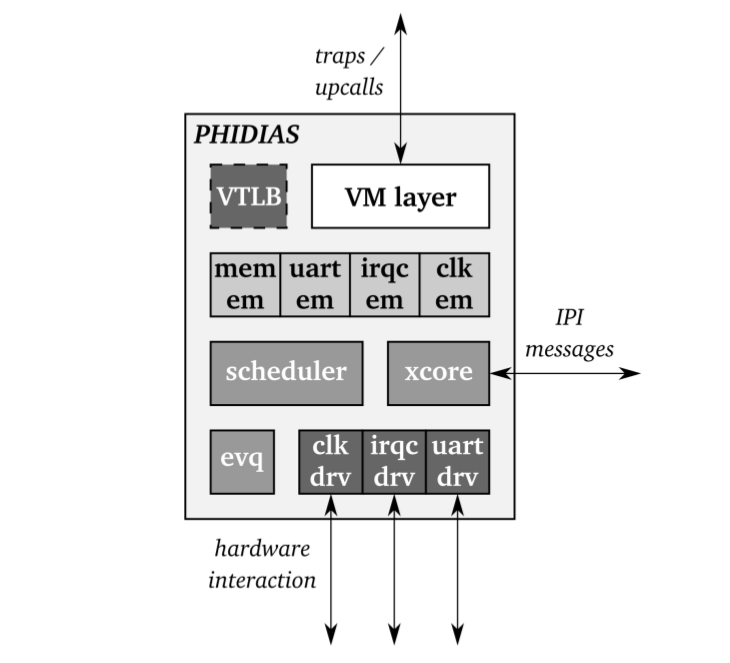
\includegraphics[width=10cm]{Phidias_Structure}
	\caption{Phidias Structure. Taken from \cite{Jan}}
	\label{Phidias_Structure}
\end{figure}

Following is a brief description for each of basic components.\\
\\
\subsubsection{VM Layer}
VM Layer is responsible for performing world switch between guests and hypervisor. It performs upcall into VM machines and dispatches events to appropriate components for handling them. 
\subsubsection{Emulation Layer}
Emulation layer consists of minimal implementation of required drivers. It includes UART, clock, Interrupt controller and a generic memory emulation. Generic memory emulation is added to run unmodified platform-specific Linux kernels without breaking their device specific functionality getting zeros on reads and writes are discarded.
\subsubsection{Scheduler and Xcore}
At the heart of PHIDIAS, there is a scheduler with simple single-priority round-robin policy and Xcore component for relaying interprocessor interrupts between different instances of hypervisor and triggering interrupt capabilities.
\subsubsection{Event Queue and Drivers for emulation}
There is an event queue which is responsible for keeping track of programmed timer events.

\subsection{Static Configuration Framework and Final Image}
Final executable image is built using a modifiable scenario specific configuration through an XML based compile time utility called Schism, the “Static Configurator for Hypervisor-Integrated Scenario Metadata”. There are two types of configuration in scenario file i.e. Hypervisor configuration and VM specific configuration.
\subsubsection{Hypervisor Configuration Elements}
\begin{itemize}
	\item Selection of CPU architecture and target platform SoC
	\item Physical and virtual Hypervisor base load address
	\item Selection of drivers for hardware devices and for the required emulation devices
\end{itemize}
\subsubsection{VM specific Configuration Elements}
\begin{itemize}
	\item Number of virtual CPUs per guest
	\item memory configuration per guest
	\item List of capabilities of each VM
	\item Assignments of pass-through interrupts to VMs
	\item Types, parameters, and corresponding emulated memory for selected emulated devices
\end{itemize}

